% ==========================================================================
% INFO 4617 Web Data Science -- Week 4: Data Formats: XML & JSON (Chapter 4)
% Build:  latexmk -pdf week-04.tex   (from this folder; no env vars needed)
% (or run `make` from the slides/ directory to build every deck)
%
% NOTE: No class Monday, Sept 7 (Labor Day). This deck runs Wednesday
% (concepts + notebook, merged into one section) and Friday (revisions).
% ==========================================================================
\documentclass[9pt,aspectratio=169]{beamer}
% Resolve the shared theme/preamble in ../common/ when compiling this
% file directly from its own folder (no TEXINPUTS needed).
\makeatletter\def\input@path{{../common/}}\makeatother
% ==========================================================================
% Shared preamble for INFO 4617 Web Data Science weekly lecture decks
% Based on the Gotham beamer theme (vendored in this directory).
% Each week's slides.tex does:  % ==========================================================================
% Shared preamble for INFO 4617 Web Data Science weekly lecture decks
% Based on the Gotham beamer theme (vendored in this directory).
% Each week's slides.tex does:  % ==========================================================================
% Shared preamble for INFO 4617 Web Data Science weekly lecture decks
% Based on the Gotham beamer theme (vendored in this directory).
% Each week's slides.tex does:  \input{preamble}  (with common/ on TEXINPUTS)
% then sets \title/\subtitle/\author/\date and \begin{document}.
% ==========================================================================

\usetheme{gotham}

\usepackage{fbb}
\usepackage{booktabs}
\usepackage{graphicx}
\usepackage{tikz}
\usepackage{xcolor}
\usepackage{multirow}
\usepackage{listings}
\usetikzlibrary{positioning, arrows.meta, shapes}

% Bibliography
\usepackage[style=authoryear,
            backend=biber,
            maxcitenames=1,
            uniquename=false,
            uniquelist=false]{biblatex}
\addbibresource{bibliography.bib}

\gothamset{sectiontocframe default=off}

% ------------------------------------------------------------------ colors
\definecolor{cugold}{HTML}{CFB87C}
\definecolor{tab-red}{HTML}{E15759}
\definecolor{tab-orange}{HTML}{F28E2B}
\definecolor{tab-blue}{HTML}{4E79A7}
\definecolor{tab-cyan}{HTML}{76B7B2}
\definecolor{tab-green}{HTML}{59A14F}
\definecolor{tab-yellow}{HTML}{EDC948}
\definecolor{tab-purple}{HTML}{B07AA1}
\definecolor{tab-pink}{HTML}{FF9DA7}
\definecolor{tab-brown}{HTML}{9C755F}
\definecolor{tab-gray}{HTML}{BAB0AC}

\setbeamercolor{frametitle}{fg=black, bg=cugold}
\setbeamercolor{progress bar}{fg=cugold, bg=cugold!20}

\setbeamercolor{block title alerted}{fg=black, bg=cugold}
\setbeamercolor{block body alerted}{fg=black, bg=cugold!10}

% ------------------------------------------------------------------ footline
\setbeamertemplate{footline}{
  \begin{beamercolorbox}[wd=\paperwidth,ht=2.5ex,dp=1ex,right]{footline}
    {\footnotesize \insertframenumber{} of \inserttotalframenumber}
    \hspace*{2ex}
  \end{beamercolorbox}
}

% ------------------------------------------------------------------ helpers
\newcommand{\bottomcite}[1]{
    \vspace*{\fill}
    \vspace{-\baselineskip}
    {\tiny
    \rule{\textwidth}{0.3pt}\\
    #1
    }
    \vspace{0.5ex}
}

% Consistent code styling for the Wednesday "applied notebook" frames.
\lstdefinestyle{wds}{
    basicstyle=\ttfamily\scriptsize,
    keywordstyle=\color{tab-blue}\bfseries,
    commentstyle=\color{tab-green},
    stringstyle=\color{tab-orange},
    showstringspaces=false,
    breaklines=true,
    columns=fullflexible,
    language=Python,
    aboveskip=0.4em,
    belowskip=0.4em,
}
\lstset{style=wds}

% \dayband{Day}{Topic} -- a lightweight section divider label used to mark
% Monday / Wednesday / Friday within a week's deck.
\newcommand{\dayband}[2]{{\large\textbf{#1}}\;\textcolor{tab-gray}{\textbar}\;#2}
  (with common/ on TEXINPUTS)
% then sets \title/\subtitle/\author/\date and \begin{document}.
% ==========================================================================

\usetheme{gotham}

\usepackage{fbb}
\usepackage{booktabs}
\usepackage{graphicx}
\usepackage{tikz}
\usepackage{xcolor}
\usepackage{multirow}
\usepackage{listings}
\usetikzlibrary{positioning, arrows.meta, shapes}

% Bibliography
\usepackage[style=authoryear,
            backend=biber,
            maxcitenames=1,
            uniquename=false,
            uniquelist=false]{biblatex}
\addbibresource{bibliography.bib}

\gothamset{sectiontocframe default=off}

% ------------------------------------------------------------------ colors
\definecolor{cugold}{HTML}{CFB87C}
\definecolor{tab-red}{HTML}{E15759}
\definecolor{tab-orange}{HTML}{F28E2B}
\definecolor{tab-blue}{HTML}{4E79A7}
\definecolor{tab-cyan}{HTML}{76B7B2}
\definecolor{tab-green}{HTML}{59A14F}
\definecolor{tab-yellow}{HTML}{EDC948}
\definecolor{tab-purple}{HTML}{B07AA1}
\definecolor{tab-pink}{HTML}{FF9DA7}
\definecolor{tab-brown}{HTML}{9C755F}
\definecolor{tab-gray}{HTML}{BAB0AC}

\setbeamercolor{frametitle}{fg=black, bg=cugold}
\setbeamercolor{progress bar}{fg=cugold, bg=cugold!20}

\setbeamercolor{block title alerted}{fg=black, bg=cugold}
\setbeamercolor{block body alerted}{fg=black, bg=cugold!10}

% ------------------------------------------------------------------ footline
\setbeamertemplate{footline}{
  \begin{beamercolorbox}[wd=\paperwidth,ht=2.5ex,dp=1ex,right]{footline}
    {\footnotesize \insertframenumber{} of \inserttotalframenumber}
    \hspace*{2ex}
  \end{beamercolorbox}
}

% ------------------------------------------------------------------ helpers
\newcommand{\bottomcite}[1]{
    \vspace*{\fill}
    \vspace{-\baselineskip}
    {\tiny
    \rule{\textwidth}{0.3pt}\\
    #1
    }
    \vspace{0.5ex}
}

% Consistent code styling for the Wednesday "applied notebook" frames.
\lstdefinestyle{wds}{
    basicstyle=\ttfamily\scriptsize,
    keywordstyle=\color{tab-blue}\bfseries,
    commentstyle=\color{tab-green},
    stringstyle=\color{tab-orange},
    showstringspaces=false,
    breaklines=true,
    columns=fullflexible,
    language=Python,
    aboveskip=0.4em,
    belowskip=0.4em,
}
\lstset{style=wds}

% \dayband{Day}{Topic} -- a lightweight section divider label used to mark
% Monday / Wednesday / Friday within a week's deck.
\newcommand{\dayband}[2]{{\large\textbf{#1}}\;\textcolor{tab-gray}{\textbar}\;#2}
  (with common/ on TEXINPUTS)
% then sets \title/\subtitle/\author/\date and \begin{document}.
% ==========================================================================

\usetheme{gotham}

\usepackage{fbb}
\usepackage{booktabs}
\usepackage{graphicx}
\usepackage{tikz}
\usepackage{xcolor}
\usepackage{multirow}
\usepackage{listings}
\usetikzlibrary{positioning, arrows.meta, shapes}

% Bibliography
\usepackage[style=authoryear,
            backend=biber,
            maxcitenames=1,
            uniquename=false,
            uniquelist=false]{biblatex}
\addbibresource{bibliography.bib}

\gothamset{sectiontocframe default=off}

% ------------------------------------------------------------------ colors
\definecolor{cugold}{HTML}{CFB87C}
\definecolor{tab-red}{HTML}{E15759}
\definecolor{tab-orange}{HTML}{F28E2B}
\definecolor{tab-blue}{HTML}{4E79A7}
\definecolor{tab-cyan}{HTML}{76B7B2}
\definecolor{tab-green}{HTML}{59A14F}
\definecolor{tab-yellow}{HTML}{EDC948}
\definecolor{tab-purple}{HTML}{B07AA1}
\definecolor{tab-pink}{HTML}{FF9DA7}
\definecolor{tab-brown}{HTML}{9C755F}
\definecolor{tab-gray}{HTML}{BAB0AC}

\setbeamercolor{frametitle}{fg=black, bg=cugold}
\setbeamercolor{progress bar}{fg=cugold, bg=cugold!20}

\setbeamercolor{block title alerted}{fg=black, bg=cugold}
\setbeamercolor{block body alerted}{fg=black, bg=cugold!10}

% ------------------------------------------------------------------ footline
\setbeamertemplate{footline}{
  \begin{beamercolorbox}[wd=\paperwidth,ht=2.5ex,dp=1ex,right]{footline}
    {\footnotesize \insertframenumber{} of \inserttotalframenumber}
    \hspace*{2ex}
  \end{beamercolorbox}
}

% ------------------------------------------------------------------ helpers
\newcommand{\bottomcite}[1]{
    \vspace*{\fill}
    \vspace{-\baselineskip}
    {\tiny
    \rule{\textwidth}{0.3pt}\\
    #1
    }
    \vspace{0.5ex}
}

% Consistent code styling for the Wednesday "applied notebook" frames.
\lstdefinestyle{wds}{
    basicstyle=\ttfamily\scriptsize,
    keywordstyle=\color{tab-blue}\bfseries,
    commentstyle=\color{tab-green},
    stringstyle=\color{tab-orange},
    showstringspaces=false,
    breaklines=true,
    columns=fullflexible,
    language=Python,
    aboveskip=0.4em,
    belowskip=0.4em,
}
\lstset{style=wds}

% \dayband{Day}{Topic} -- a lightweight section divider label used to mark
% Monday / Wednesday / Friday within a week's deck.
\newcommand{\dayband}[2]{{\large\textbf{#1}}\;\textcolor{tab-gray}{\textbar}\;#2}


\title[Week 4 · Data Formats]{{\Huge Data Formats: XML \& JSON}}
\subtitle{Week 4 · Foundations module · Textbook Chapter 4}
\author[Keegan]{\textbf{Brian C. Keegan, Ph.D.} \\ Associate Professor, Department of Information Science \\ University of Colorado Boulder}
\date{September 9 \& 11, 2026}

\begin{document}

\maketitle

% -------------------------------------------------------------------------
\begin{frame}{This week at a glance}
    \begin{columns}[T]
        \begin{column}{0.6\textwidth}
            Two formats carry almost all web data: \textbf{XML} (a tree of tags) and \textbf{JSON} (nested lists and dictionaries).

            \bigskip

            \dayband{Monday}{Labor Day --- no class}
            \begin{itemize}\small
                \item Monday's concept intro is folded into Wednesday
            \end{itemize}

            \medskip

            \dayband{Wednesday}{Concepts \& notebook lab}
            \begin{itemize}\small
                \item XML \& JSON concepts, then the Chapter 4 notebook: Congress, tweets, and weather
            \end{itemize}

            \medskip

            \dayband{Friday}{Textbook revisions}
            \begin{itemize}\small
                \item Propose \& peer-review pull requests from Chapters 1--4
            \end{itemize}
        \end{column}
        \begin{column}{0.35\textwidth}
            \begin{block}{Companion notebook}
                \footnotesize \texttt{ch-04-data-formats.ipynb}
            \end{block}
        \end{column}
    \end{columns}
\end{frame}

\begin{frame}{Daily note questions}
    \begin{itemize}\small 
        \item \textbf{What happens if an issue is resolved incorrectly?} --- GitHub is primarily a version control system, so it is possible to ``rewind'' to an earlier version. In other words, don't stress you'll ``break'' something.
        \item \textbf{Don't understand how to file a pull request.} --- We'll keep practicing more this Friday, I need to do more scaffold a good example.
        \item \textbf{Concerns with citing information added to textbook?} --- You should all have ``write'' access to merge pull requests right away, which will update the textbook for everyone.
        \item \textbf{Will all issues eventually be merged?} --- Probably not, but that isn't what you're graded on.
    \end{itemize}
\end{frame}

% =========================================================================
\section{Wednesday · Concepts \& Notebook}
% =========================================================================

\begin{frame}{The role of data formats}
    \begin{columns}[T]
        \begin{column}{0.6\textwidth}
            Two formats dominate data from the web:

            \medskip
            \begin{itemize}\small
                \item \textbf{XML} --- the older format and a down-payment on HTML: a tree of nested tags.
                \item \textbf{JSON} --- the newer, lighter format of the API economy: lists and dictionaries.
            \end{itemize}

            \medskip
            Every page, API response, and data feed you meet this semester is going to be a flavor of XML or JSON
        \end{column}
        \begin{column}{0.35\textwidth}
            \begin{block}{When to use which}
                \footnotesize
                \textbf{XML}: older web services, government feeds (Congress, SEC, RSS), configuration files.

                \medskip
                \textbf{JSON}: modern web APIs, database exports, service-to-service exchange.
            \end{block}
        \end{column}
    \end{columns}
\end{frame}

\begin{frame}{A brief history of XML}
    \begin{columns}[T]
        \begin{column}{0.6\textwidth}
            XML and HTML are often assumed to be one a subset of the other, but they are siblings descending from SGML
            
            \medskip
            The HTML you scrape in the wild almost never is valid XML, need a different more generous parser

            \medskip
            XML is a foundation for a whole family of other languages: XHTML (websites), SVG (images), MathML (math equations), RSS (podcasts)

            \medskip
            XML hides in plain sight: open a \texttt{.docx}, \texttt{.xlsx}, or \texttt{.svg} file's internals and you are looking at it.
        \end{column}
        \begin{column}{0.35\textwidth}
            
\includegraphics[width=\textwidth]{slides/week-04/img/zip-folders.png}
        \end{column}
    \end{columns}
\end{frame}

\begin{frame}{A brief history of JSON}
    \begin{columns}[T]
        \begin{column}{0.6\textwidth}
            JSON specified in the early 2000s

            \medskip
            JSON's design goal was the opposite of XML's: no tags, no schema, no comments --- ``just the data''
            
            \medskip
            Objects and arrays that can be recognized by all modern programming languages and easy for machines to parse

            \medskip
            As Python-native coders, JSON intuitively matches lists and dictionaries you already know
        \end{column}
        \begin{column}{0.35\textwidth}
            
\includegraphics[width=\textwidth]{slides/week-04/img/json-statham.jpg}
        \end{column}
    \end{columns}
\end{frame}

\begin{frame}[fragile]{XML: a tree of nested tags}
    XML organizes data as a \textbf{hierarchy}: each tag can hold text, attributes, and child tags. The House \texttt{MemberData} feed, drawn as a tree:
\begin{lstlisting}[basicstyle=\large\ttfamily]
<MemberData>
  <member>                     # repeats 441 times
    <member-info>
      <firstname>Joe</firstname>     # value in TEXT
      <lastname>Neguse</lastname>
      <party>D</party>
    </member-info>
    <state postal-code="CO">         # value in an ATTRIBUTE
      <state-fullname>Colorado</state-fullname>
    </state>
  </member>
</MemberData>
\end{lstlisting}
    A value hides in one of two places: \textbf{text} (read with \texttt{.text}) or an \textbf{attribute} (read with brackets).
\end{frame}

\begin{frame}[fragile]{JSON: lists and dictionaries you already know}
    JSON maps onto two Python structures you already use. The weather forecast, peeled one layer at a time:
\begin{lstlisting}[basicstyle=\large\ttfamily]
{                              # dict: type(data) is dict
  "latitude": 40.01,
  "daily": {                    # dict: data["daily"]
    "time": [...],               # list: data["daily"]["time"]
    "temperature_2m_max": [...]
  }
}
\end{lstlisting}
    A JSON \textbf{array} is a Python \textbf{list}; a JSON \textbf{object} is a Python \textbf{dict}. Real data nests them several levels deep --- the skill is navigating from the outside in, one \texttt{type()} and \texttt{.keys()} call at a time.
\end{frame}

\begin{frame}{JSON vs.\ XML: pick your trade-offs}
    \begin{columns}[T]
        \begin{column}{0.48\textwidth}
            \begin{block}{JSON}
                \small
                \textbf{+} Compact --- no repeated tag names

                \textbf{+} Parses natively in JavaScript

                \textbf{+} Simple: objects, arrays, 4 scalar types

                \textbf{--} No comments allowed

                \textbf{--} No native schema enforcement

                \textbf{--} No display semantics --- data only
            \end{block}
        \end{column}
        \begin{column}{0.48\textwidth}
            \begin{block}{XML}
                \small
                \textbf{+} Schema validation (DTD/XSD) before parsing

                \textbf{+} Rich vocabulary: attributes, mixed content, namespaces

                \textbf{+} Can double as a document format (SVG, DOCX)

                \textbf{--} Verbose --- every tag closes

                \textbf{--} No native browser/JS parsing

                \textbf{--} Everything parses as text; you convert types
            \end{block}
        \end{column}
    \end{columns}
    \medskip
    \centering\small Neither is intrinsically better than the other --- just different tools for different needs
\end{frame}

\begin{frame}{Where JSON and XML show up}
    \begin{columns}[T]
        \begin{column}{0.6\textwidth}
            JSON dominates anywhere a \textbf{program} is the primary reader, particularly APIs

            \medskip
            XML persists where a human sometimes needs to read the document, where a strict contract matters, or where the data predates the JSON era.

            \medskip
            Government and legislative systems still commonly use XML --- partly because XSD validation guarantees a submitted document has the fields it is supposed to have.
        \end{column}
        \begin{column}{0.35\textwidth}
            \begin{alertblock}{Rule of thumb}
                \footnotesize 
                If a program wrote it and a program will read it, expect JSON.

                \medskip
                If humans are involved in read/write or high-stakes data, expect XML.
            \end{alertblock}
        \end{column}
    \end{columns}
\end{frame}

\begin{frame}{Common pipeline}

            Whether data starts as XML, JSON, HTML, or PDF text, the move into analysis is always the same:

            \medskip
            \begin{center}
                \textbf{find records} $\rightarrow$ \textbf{extract fields} $\rightarrow$ \textbf{\texttt{lists} + \texttt{dicts}} $\rightarrow$ \texttt{pd.DataFrame}
            \end{center}

            \medskip
            Once you are in a DataFrame, a whole host of other data science methods for cleaning, filtering, grouping, aggregating, merging open up
\end{frame}

\begin{frame}[fragile]{Parsing XML with BeautifulSoup}
    Parse the string into a navigable tree, then search it. \texttt{.find()} returns the first match, \texttt{.find\_all()} returns them all --- each searches the \textit{entire} subtree beneath a tag:
\begin{lstlisting}[basicstyle=\small\ttfamily]
from bs4 import BeautifulSoup

soup = BeautifulSoup(house_raw, "xml")   # the "xml" parser comes from lxml

members = soup.find_all("member")
print(len(members))                       # 2

for m in members:
    first = m.find("firstname").text      # .text = content between the tags
    last  = m.find("lastname").text       # .find() reaches nested tags too
    party = m.find("party").text
    print(f"{first} {last} ({party})")    # Joe Neguse (D) / Jeff Hurd (R)
\end{lstlisting}
\end{frame}

\begin{frame}[fragile]{Data exists in two different places in XML}
    \begin{columns}[T]
        \begin{column}{0.6\textwidth}
            A value is either \textbf{text} or an \textbf{attribute}:
\begin{lstlisting}[basicstyle=\small\ttfamily]
state = soup.find("state")
state["postal-code"]                # "CO"
state.find("state-fullname").text   # "Colorado"
\end{lstlisting}
            
            \bigskip
            A missing tag makes \texttt{.find()} return \texttt{None}:
\begin{lstlisting}[basicstyle=\small\ttfamily]
# AttributeError: None has no .text
m.find("party").text
# guard every extraction instead:
m.find("party").text if m.find("party") else None
\end{lstlisting}
        \end{column}
        \begin{column}{0.35\textwidth}
            Working out \textit{which} of the two holds your value is half the parsing battle --- real XML uses both.

            \bigskip

            Calling \texttt{.text} on a \texttt{None} is the \textbf{single most common} scraping error. The \texttt{if \dots else None} guard keeps one missing field from crashing a 441-record loop.

            \bigskip

            XML always hands you \textbf{text}: converting \texttt{"2nd"} or \texttt{"\$1,234"} to a number is your job.
        \end{column}
    \end{columns}
\end{frame}

\begin{frame}[fragile]{XML $\rightarrow$ DataFrame: the real House roster}
    \begin{columns}[T]
        \begin{column}{0.55\textwidth}
\begin{lstlisting}[basicstyle=\footnotesize\ttfamily]
import requests, pandas as pd

url = "https://clerk.house.gov/xml/lists/MemberData.xml"
soup = BeautifulSoup(requests.get(url).text, "xml")
print(soup.find("MemberData")["publish-date"])

records = []
for m in soup.find_all("member"):    # 441 members
    st = m.find("state")
    records.append({"last_name": m.find("lastname").text,
                    "party": m.find("party").text,
                    "state": st["postal-code"] if st else None})
df = pd.DataFrame(records)   # find_all -> dicts -> DataFrame
\end{lstlisting}
        \end{column}
        \begin{column}{0.42\textwidth}
            \textbf{\footnotesize The raw response, before parsing:}
\begin{lstlisting}[basicstyle=\footnotesize\ttfamily]
July 1, 2026
<member>
 <member-info>
  <firstname>Joe</firstname>
  <lastname>Neguse</lastname>
  <party>D</party>
 </member-info>
 <state postal-code="CO">
  <state-fullname>
   Colorado
  </state-fullname>
 </state>
</member>
\end{lstlisting}
        \end{column}
    \end{columns}
\end{frame}

\begin{frame}[fragile]{JSON: parse a string, then the list-of-dictionaries pipeline}
    \texttt{json.loads()} turns a \textbf{s}tring into Python objects (\texttt{json.load()} reads a \textbf{f}ile). With \texttt{requests}, \texttt{response.json()} does it for you:
\begin{lstlisting}[basicstyle=\small\ttfamily]
import json, pandas as pd

data = json.loads('{"state": "Colorado", "population": 5773714}')
print(data["state"])              # Colorado
# response.json()  ==  json.loads(response.text)

census = [                        # the list-of-dictionaries pattern:
    {"state": "Colorado", "year": 2020, "population": 5773714},
    {"state": "Colorado", "year": 2010, "population": 5029196},
]
df = pd.DataFrame(census)         # one dict per row, keys -> columns
\end{lstlisting}
\end{frame}

\begin{frame}[fragile]{JSON: peel the onion on a live API}
    \begin{columns}[T]
        \begin{column}{0.6\textwidth}
\begin{lstlisting}[basicstyle=\small\ttfamily]
import requests

url = "https://api.open-meteo.com/v1/forecast"
params = {"latitude": 40.01, "longitude": -105.27,
          "daily": "temperature_2m_max",
          "timezone": "America/Denver"}
data = requests.get(url, params=params).json()

# type() + .keys(), one level deeper each time
data.keys()            # latitude, longitude, daily...
data["daily"].keys()   # time, temperature_2m_max
highs = data["daily"]["temperature_2m_max"]  # a list
data.get("elevation", "unknown")  # .get avoids KeyError
\end{lstlisting}
        \end{column}
        \begin{column}{0.35\textwidth}
            \centering
            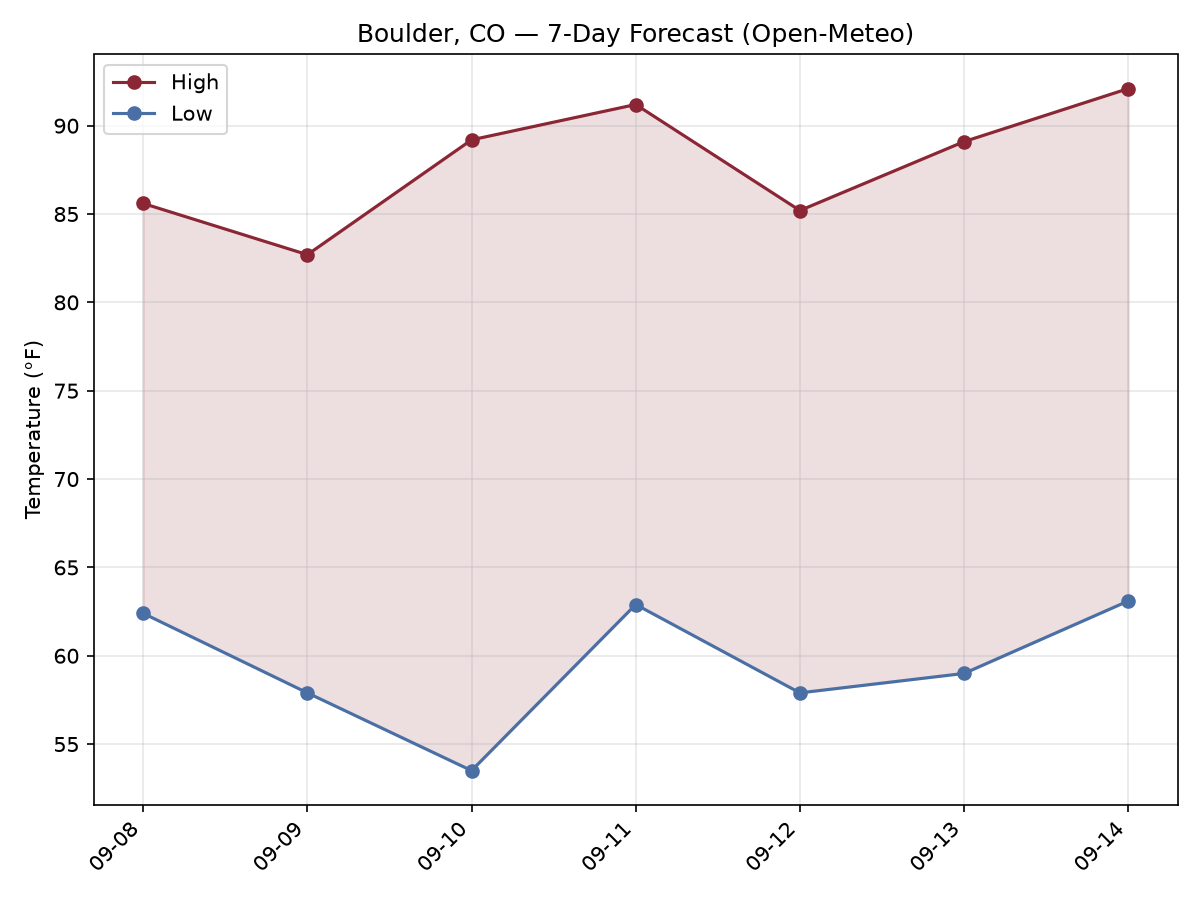
\includegraphics[width=\textwidth]{img/weather_forecast_plot.png}\\
            {\scriptsize Boulder's 7-day forecast, fetched live on Sept.~8.}
        \end{column}
    \end{columns}
\end{frame}

\begin{frame}{Lab: work these in pairs, then show-and-tell}
    \begin{columns}[T]
        \begin{column}{0.6\textwidth}
            Work in pairs. Do these exercises from the Chapter 4 notebook:
            \begin{enumerate}\small
                \item \textbf{RSS feed} --- parse a news feed with the \texttt{"xml"} parser. Extract the title, the link, and the date. Put them in a DataFrame.
                \item \textbf{Nested JSON} --- get the dates and the maximum temperatures from Open-Meteo. Put them in a DataFrame.
                \item \textbf{XML and JSON} --- get the same data in both formats. Report which format is easier to parse. Report which format has more metadata.
                \item \textbf{Reusable} --- write \texttt{xml\_to\_dataframe(soup, tag, fields)}. Test it on the Congress data. Then test it on an RSS feed.
                \item \textbf{Weather} --- plot the high and low temperatures. Mark the days below freezing.
                \item[6.] \textbf{5617}: write a critique of a public XML or JSON dataset. Use the datasheet format of \textcite{gebru2021datasheets}
            \end{enumerate}
        \end{column}
        \begin{column}{0.35\textwidth}
            \begin{block}{Show-and-Tell}
                \footnotesize Bring one of these to class:
                \begin{itemize}\footnotesize
                    \item a bug that you could not solve
                    \item data that you collected and find interesting
                    \item a question for a research design
                \end{itemize}
            \end{block}
            \begin{alertblock}{Error flavors}
                \footnotesize Some code here is \textit{designed} to break (a guard demonstrating a crash) --- that does not need a GitHub issue. Other code may be \textit{genuinely} broken: confirm it, then search and file an issue.
            \end{alertblock}
        \end{column}
    \end{columns}
\end{frame}

\begin{frame}{Effort over perfection}
    \begin{columns}[T]
        \begin{column}{0.6\textwidth}
            Start the lab in class, finish at home, submit what you got working. Graded on a good-faith attempt to complete the notebook, not on getting every cell to run.
        \end{column}
        \begin{column}{0.35\textwidth}
            \begin{block}{Submitting}
                \footnotesize Run all cells, then export: \textit{File $\rightarrow$ Save and Export Notebook As $\rightarrow$ HTML}. Upload to Canvas by \textbf{Sunday 11:59pm}.
            \end{block}
        \end{column}
    \end{columns}
\end{frame}

% =========================================================================
\section{Friday · Textbook Revisions}
% =========================================================================

\begin{frame}{A worked example --- linking the Missing Manual}
    \begin{columns}[T]
        \begin{column}{0.6\textwidth}
            Until this week, \texttt{ch-04-data-formats.qmd} had this line:

            \medskip
            \textit{``For more on data file formats\ldots{} see Missing Manual Chapter 20: Data File Formats.''}

            \medskip
            It named a chapter. It didn't link to it. A reader had to leave the page, find the Missing Manual site, and search for Chapter 20 by hand.

            \medskip
            Here's exactly how that got fixed --- eight steps, start to finish. Yours will be a different gap; the mechanics are identical.
        \end{column}
        \begin{column}{0.35\textwidth}
            \begin{alertblock}{The target}
                \footnotesize \url{https://cuinfoscience.github.io/INFO-Missing-Manual/chapters/data-file-formats.html}
            \end{alertblock}
        \end{column}
    \end{columns}
\end{frame}

\begin{frame}{Step 1 --- find the file}
    \begin{columns}[T]
        \begin{column}{0.6\textwidth}
            Two ways in:
            \begin{enumerate}\small
                \item Open the rendered chapter. Click \textbf{Edit this page} in the sidebar.
                \item Or browse the repo directly: \texttt{cuinfoscience/Web-Data-Science-Book}, then open \texttt{ch-04-data-formats.qmd}.
            \end{enumerate}

            \medskip
            Both paths land on the same page: the raw \texttt{.qmd} source, in GitHub's file viewer.
        \end{column}
        \begin{column}{0.35\textwidth}
            \begin{alertblock}{Edit the right file}
                \footnotesize The \texttt{.qmd} is the source. Never the rendered HTML, and never the \texttt{.ipynb} --- it is generated from the chapter, and your edit would be overwritten.
            \end{alertblock}
        \end{column}
    \end{columns}
\end{frame}

\begin{frame}{Step 2 --- open the editor}
    \begin{columns}[T]
        \begin{column}{0.6\textwidth}
            Click the pencil icon in the top right of the file view --- \textbf{Edit this file}.

            \medskip
            You have write access now. GitHub takes you straight into an in-browser text editor. No fork, no separate copy --- you are editing the real repository.
        \end{column}
        \begin{column}{0.35\textwidth}
            \begin{alertblock}{One change per PR}
                \footnotesize A PR is a conversation about one change. Add one link today, not everything you happen to notice.
            \end{alertblock}
        \end{column}
    \end{columns}
\end{frame}

\begin{frame}{Step 3 --- find the line}
    \begin{columns}[T]
        \begin{column}{0.6\textwidth}
            The chapter runs past 500 lines. Do not scroll to find one sentence.

            \medskip
            Click inside the editor. Press \textbf{Ctrl+F} (\textbf{Cmd+F} on a Mac) to open the editor's own search bar.

            \medskip
            Search for \texttt{Missing Manual Reference}. It appears once, near the end of the chapter.
        \end{column}
        \begin{column}{0.35\textwidth}
            \begin{alertblock}{The wrong search bar still works, badly}
                \footnotesize Your browser's Ctrl+F only searches what is currently rendered. GitHub's editor holds the whole file. Search inside the editor pane, not the page.
            \end{alertblock}
        \end{column}
    \end{columns}
\end{frame}

\begin{frame}[fragile]{Step 4 --- write the Markdown link}
    A Markdown link has the form \texttt{[text](url)}. Wrap the existing phrase --- do not retype it:
\begin{lstlisting}[language=,basicstyle=\ttfamily\small]
Before:
...see *Missing Manual* Chapter 20: Data File Formats.

After:
...see [*Missing Manual* Chapter 20: Data File Formats]
(https://cuinfoscience.github.io/INFO-Missing-Manual/
chapters/data-file-formats.html).
\end{lstlisting}
    The italics markup stays inside the brackets. Link text can carry other formatting.
\end{frame}

\begin{frame}{Step 5 --- preview it}
    \begin{columns}[T]
        \begin{column}{0.6\textwidth}
            Click the \textbf{Preview} tab above the editor.

            \medskip
            Check three things:
            \begin{enumerate}\small
                \item The phrase is blue and underlined --- a live link.
                \item The italics survived --- \textit{Missing Manual} still reads in italics.
                \item Nothing else on the page changed.
            \end{enumerate}
        \end{column}
        \begin{column}{0.35\textwidth}
            \begin{alertblock}{Do not click the link yet}
                \footnotesize Verify it visually first. Test that it actually resolves after the PR's render check runs.
            \end{alertblock}
        \end{column}
    \end{columns}
\end{frame}

\begin{frame}{Step 6 --- commit to a new branch}
    \begin{columns}[T]
        \begin{column}{0.6\textwidth}
            Scroll down. Below the editor, GitHub asks how to save your change.

            \medskip
            Write a short commit title: \textit{``Link the Missing Manual chapter reference in Ch.~4.''}

            \medskip
            Select \textbf{Create a new branch for this commit and start a pull request} --- not \textit{Commit directly to the main branch}.
        \end{column}
        \begin{column}{0.35\textwidth}
            \begin{alertblock}{Write access is not a shortcut}
                \footnotesize You can push straight to \texttt{main}. That does not mean you should. A branch gives a reviewer something to read before it ships.
            \end{alertblock}
        \end{column}
    \end{columns}
\end{frame}

\begin{frame}{Step 7 --- open the pull request}
    Click \textbf{Propose changes}.

    \medskip
    GitHub moves you to the \textbf{Comparing changes} screen: your branch on the left, \texttt{main} on the right, the diff in between.

    \medskip
    Check the diff. One line removed, one line added, nothing else. That is what ``one change per PR'' looks like on screen, not just in principle.

    \medskip
    Click \textbf{Create pull request} to open the title and description form.
\end{frame}

\begin{frame}[fragile]{Step 8 --- write a good description}
    Use the same four fields as your issues, now describing a fix instead of a problem:
\begin{lstlisting}[language=,basicstyle=\ttfamily\footnotesize]
Location: ch-04-data-formats.qmd, "Missing Manual Reference"

Problem:  The callout names Chapter 20 but gives no way to
          click through to it.

Why:      A reader has to leave the page and search the
          Missing Manual site by hand to find the chapter.

Change:   Wrapped the existing text in a Markdown link to
          the chapter's page.
\end{lstlisting}
    Click \textbf{Create pull request}. Your PR is open.
\end{frame}

\begin{frame}{What happens next}
    \begin{columns}[T]
        \begin{column}{0.6\textwidth}
            Every PR against the book triggers a render check. Green means the book still builds with your change. Red means read the log before asking --- the failing line is usually named.

            \medskip
            Watch for a reviewer's comments. Push a follow-up commit to the same branch if asked, or defend your choice.

            \medskip
            When it merges, the book republishes itself. Reload the chapter in a few minutes --- your fix is live, the same way this one is.
        \end{column}
        \begin{column}{0.35\textwidth}
            \begin{alertblock}{The loop you're about to close}
                \footnotesize Reader $\rightarrow$ found a gap $\rightarrow$ edited $\rightarrow$ opened a PR $\rightarrow$ merged $\rightarrow$ live page. All of it in a browser tab.
            \end{alertblock}
        \end{column}
    \end{columns}
\end{frame}

\begin{frame}{A revision menu for Chapter 4}
    High-value targets --- pick one and scope it to a single PR:
    \begin{itemize}
        \item \textbf{Test the code against live sources.} The House roster drifts (441 today; the \texttt{publish-date} changes) and Open-Meteo dates roll forward. Run the notebook, report what changed, and pin the snapshot.
        \item \textbf{Close a gap in ``Common Issues to Debug.''} Add a worked \texttt{json.JSONDecodeError} case --- a trailing comma, single quotes, or an HTML error page returned instead of JSON.
        \item \textbf{Verify a real-world-patterns claim.} The chapter names specific places JSON and XML show up (JWTs, SOAP, Office file formats). Check one against a primary source and tighten the citation.
        \item \textbf{Strengthen an exercise.} Give the RSS or weather exercise expected output, a rubric, or a starter cell so it is self-checking.
        \item \textbf{Extend the RSS / post-API story.} Tie the decline-of-RSS narrative to a concrete citation and the ``soft enclosure'' theme (Ch.~3).
    \end{itemize}
\end{frame}

\begin{frame}{A good revision, and a good review}
    \begin{columns}[T]
        \begin{column}{0.45\textwidth}
            \begin{block}{A strong PR}
                \begin{itemize}\small
                    \item One focused change, clearly titled
                    \item Explains the problem it fixes
                    \item Renders (\texttt{quarto render}) without errors
                    \item Matches the book's voice and notation
                    \item Discloses any AI assistance
                \end{itemize}
            \end{block}
        \end{column}
        \begin{column}{0.45\textwidth}
            \begin{block}{A strong review}
                \begin{itemize}\small
                    \item Runs / reads the change, not just skims
                    \item Names specifics (line, claim, code)
                    \item Separates ``must fix'' from ``nice to have''
                    \item Is generous --- assume good faith
                    \item Ends with a clear verdict
                \end{itemize}
            \end{block}
        \end{column}
    \end{columns}
    \medskip
    \centering\small Next week: \textbf{Web Architecture \& Protocols} --- how a URL becomes a rendered page (HTTP, requests, status codes).
\end{frame}

\begin{frame}[fragile]{The reviewer's tool --- a suggestion}
    \begin{columns}[T]
        \begin{column}{0.55\textwidth}
            Reviewing someone else's PR? Do not just describe the fix in a comment. Propose it directly:
\begin{lstlisting}[language=,basicstyle=\ttfamily\footnotesize]
```suggestion
XML 1.0 became a W3C
Recommendation in 1998.
```
\end{lstlisting}
        \end{column}
        \begin{column}{0.4\textwidth}
            One click for the author to accept it. This is the fastest way to turn ``must fix'' into a merged change.
        \end{column}
    \end{columns}
\end{frame}

% =========================================================================
\begin{frame}{Key takeaways}
    \begin{enumerate}
        \item \textbf{XML} is a tree of tags; \textbf{JSON} is nested lists and dictionaries --- the two structural languages of web data.
        \item XML (1998, from SGML) favors strict contracts and documents a human might read; JSON (early 2000s, from JavaScript) favors compact, program-to-program exchange.
        \item BeautifulSoup navigates XML with \texttt{.find()}, \texttt{.find\_all()}, and \texttt{.text}; attributes come out with bracket notation. For JSON, \textbf{peel the onion} --- \texttt{type()} and \texttt{.keys()}, top-down.
        \item The \texttt{find\_all} $\rightarrow$ list-of-dicts $\rightarrow$ \texttt{DataFrame} pipeline is the bridge from raw web data to analysis.
        \item Format is a \textbf{transparency} choice: open XML and JSON support public oversight; scanned PDFs prevent it.
    \end{enumerate}
\end{frame}

\end{document}
